\chapter{Szimulációk}
A teljes struktúrát együttesen nem szimuláltam le, mivel az egyes alkotóelemek méretezését külön-külön végeztem első körben, de még nem minddel jutottam értékelhető eredményre. A differenciális vonallal és az antennával sikerült teljesítenem a követelményeket, a balun és a földkitöltés szélén az áramblokkoló mintázat még nincs használható állapotban.
\par Az balunnal egyszerűen nem teljesült a maximum -10 dB-s bemeneti (CPW) reflexiós követelmény a kimenet (CPS) illesztett lezárása mellett. Az áramblokkoló mintázat tervezésével pedig azért nem foglalkoztam, mert ennek a vizsgálatához érdemes a többi komponenst elfogadhatóan megtervezni, mivel ez a mintázat gyakorlatilag csak az antenna sugárzási karakterisztikáját kell, hogy befolyásolja. Ugyan a földkitöltés viselkedése az antenna bemeneti impedanciáját is befolyásolja, de feltehetőleg csak olyan mértékben, hogy az az antenna paramétereinek enyhe változtatásával az újból kihangolható.
\par A legjobb szimulált balun bemeneti reflexió \aref{fig:balun-s11}. ábrán látható, a szimulációhoz a balun keresztmetszetei \aref{fig:balun-kereszt}. ábrán, a balun méretparaméterei pedig \aref{tab:balun-param}. táblázatban láthatóak.
\begin{figure}[h]
	\centering
	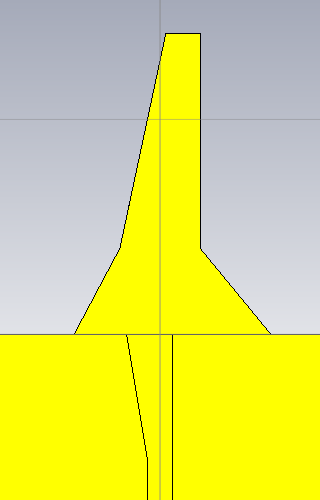
\includegraphics[width=0.6\textwidth]{kep/results/balun_1.bmp}
	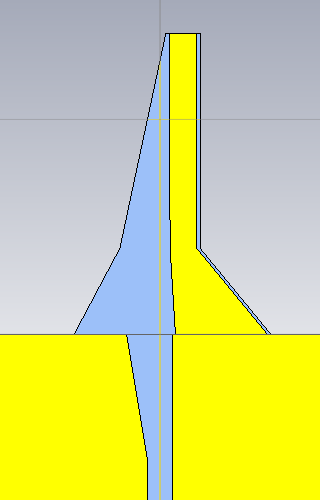
\includegraphics[width=0.6\textwidth]{kep/results/balun_2.bmp}
	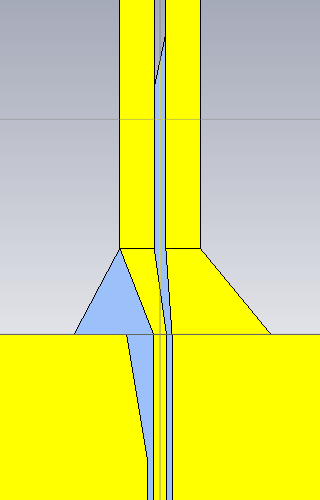
\includegraphics[width=0.6\textwidth]{kep/results/balun_3.bmp}
	\caption{A szimulált balun struktúra keresztmetszetei.}
	\label{fig:balun-kereszt}
\end{figure}
\begin{figure}[h]
	\centering
	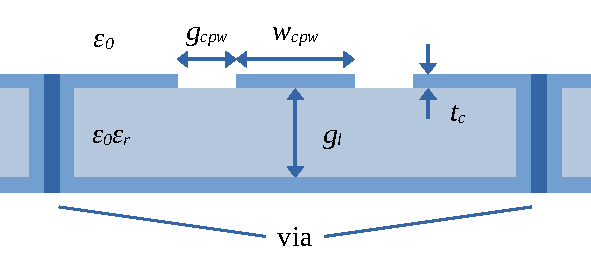
\includegraphics[width=0.6\textwidth]{kep/cpw.pdf}
	\caption{A rádió felől érkező koplanár tápvonal (CPW) keresztmetszete.}
	\label{fig:balun-s11}
\end{figure}
\begin{table}[h!]
	\centering
	\begin{tabular}{||c|c|c|c|c||c|c||}
	\hline
	$\varepsilon_r$ & $t_{sub}$ & $t_{c}$ & $g_{cps}$ & $w_{cps}$ & $Z_{c}$ & $Z_{slotline}$ \\ [0.5ex] 
	\hline\hline
	4,3 & \SI{1,55}{mm} & \SI{0,03}{mm} & \SI{0,274}{mm} & \SI{0,8}{mm} & \SI{100,19}{\ohm} & \SI{74,4}{\ohm}\\
	\hline
	\end{tabular}
	\caption{asd}
	\label{tab:balun-param}
\end{table}